\documentclass{beamer}
\usetheme{Madrid}
\usecolortheme{default}
\usepackage{amsmath}
\usepackage{tikz}
\usetikzlibrary{arrows.meta}
\usetikzlibrary{angles, quotes}


\title{Relative Motion in 2D}
\subtitle{SPH3UI - Day 2}
\author{}
\date{}

\begin{document}

\begin{frame}
\titlepage
\end{frame}

\begin{frame}{Relative Motion in 2D}
\begin{center}
\Large What if our reference planes are not parallel to one another?
\end{center}
\end{frame}

\begin{frame}{Introduction}
\textbf{Previously}, we examined motion involving two objects moving relative to one another in one plane, where vector addition was (somewhat) intuitive.
 
\vspace{0.5cm}

\textbf{Today}, we will extend this idea to situations where the two objects move in different planes. For example, motion of one object is perpendicular to or at an angle from the direction of motion of the other object.
 
\vspace{0.5cm}

This topic is characterized by the classic \textbf{river crossing problem.}
\end{frame}

\begin{frame}{Example 1: No Current}
\textbf{Problem:} A physics student steers straight across a river at 12 km/h [N] to get to school. If the river is 0.30 km across with no current, how long will it take her to cross the river?
 
\vspace{0.3cm}

\textbf{Given:} 
\begin{itemize}
\item \(\Delta d_y = 0.30\) km [N]
\item \(v_y = 12\) km/h [N]
\end{itemize}
 

\textbf{Required:} \(\Delta t\)
 

\vspace{0.3cm}

\textbf{Analysis:} 
 
\[v_y = \frac{\Delta d_y}{\Delta t} \Rightarrow \Delta t = \frac{\Delta d_y}{v_y}\]
\end{frame}

\begin{frame}{Example 1: No Current (continued)}
\textbf{Solution:}
 
\[\Delta t = \frac{0.30 \text{ km}}{12 \text{ km/h}} = 0.025 \text{ h}\]
 
\[\Delta t = 0.025 \text{ h} \times \frac{60 \text{ min}}{1 \text{ hour}} = 1.5 \text{ min}\]
 

\vspace{0.5cm}
\begin{center}
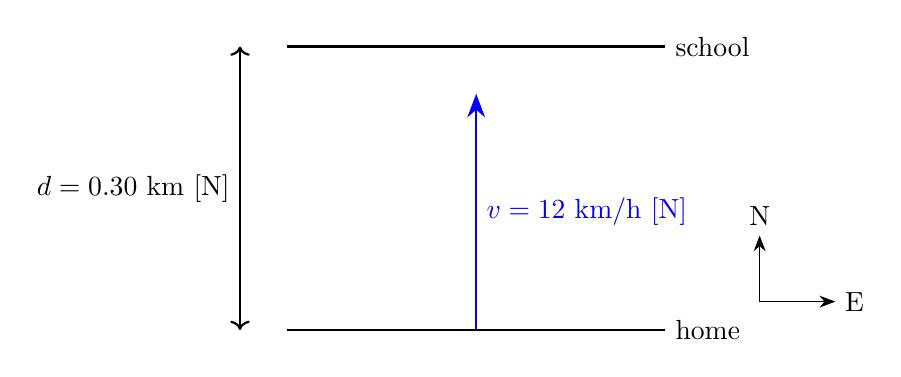
\begin{tikzpicture}[scale=1.2]
\draw[thick] (0,0) -- (4,0) node[right] {home};
\draw[thick] (0,3) -- (4,3) node[right] {school};
\draw[-{Stealth[length=3mm]}, thick, blue] (2,0) -- (2,2.5) node[midway, right] {\(v = 12\) km/h [N]};
 
\draw[<->, thick] (-0.5,0) -- (-0.5,3) node[midway, left] {\(d = 0.30\) km [N]};
\draw[-{Stealth[length=2mm]}] (5.0,0.3) -- (5.8,0.3) node[right] {E};
\draw[-{Stealth[length=2mm]}] (5.0,0.3) -- (5.0,1) node[above] {N};
\end{tikzpicture}
\end{center}
\end{frame}

\begin{frame}{Example 2: Perpendicular Current}
\textbf{Problem:} Another day, the same physics student wants to cross the river, but this time, it is far windier. The river water now flows with a current of 24 km/h [E].
 
\vspace{0.3cm}

\textbf{a) How long does it take to cross the river?}
 
\vspace{0.3cm}

\textbf{Given:}
\begin{itemize}
\item \(v_y = 12\) km/h [N]
\item \(v_x = 24\) km/h [E]
\item \(\Delta d_y = 0.30\) km [N]
\end{itemize}
 

\textbf{Required:} \(\Delta t\)
 
\vspace{0.3cm}

\textbf{Analysis:} 
 
\[v_y = \frac{\Delta d_y}{\Delta t} \Rightarrow \Delta t = \frac{\Delta d_y}{v_y}\]
\end{frame}

\begin{frame}{Example 2: Perpendicular Current (continued)}
\textbf{Solution:}
 
\[\Delta t = \frac{0.30 \text{ km}}{12 \text{ km/h}} = 0.025 \text{ h}\]
 

\textbf{Important:} Since there is no change to the motion in the y-direction, the time it takes to cross the river is the same as when there was no current!
 
\vspace{0.3cm}

\begin{center}
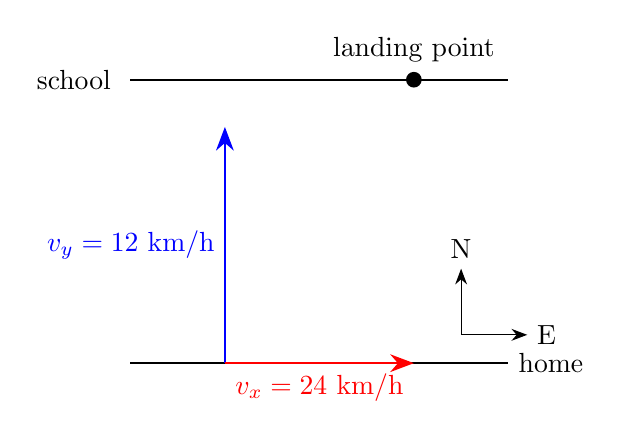
\begin{tikzpicture}[scale=1.2]
\draw[thick] (0,0) -- (4,0) node[right] {home};
\draw[thick] (0,3) -- (4,3);
 
\draw[-{Stealth[length=3mm]}, thick, blue] (1,0) -- (1,2.5) node[midway, left] {\(v_y = 12\) km/h};
 
\draw[-{Stealth[length=3mm]}, thick, red] (1,0) -- (3,0) node[midway, below] {\(v_x = 24\) km/h};
\node at (3,3) [circle, fill=black, inner sep=2pt, label=above:landing point] {};
\node at (0,3) [label=left:school] {};
\draw[-{Stealth[length=2mm]}] (3.5,0.3) -- (4.2,0.3) node[right] {E};
\draw[-{Stealth[length=2mm]}] (3.5,0.3) -- (3.5,1) node[above] {N};
\end{tikzpicture}
\end{center}
\end{frame}

\begin{frame}{Example 2: Perpendicular Current}
\textbf{b) How far downstream does the boat travel before it reaches the shore?}
 
\vspace{0.3cm}

\textbf{Given:}
\begin{itemize}
\item \(v_x = 24\) km/h [E]
\item \(\Delta t = 0.025\) h
\end{itemize}
 

\textbf{Required:} \(\Delta d_x\)
 
\vspace{0.3cm}

\textbf{Analysis:} 
 
\[v_x = \frac{\Delta d_x}{\Delta t} \Rightarrow \Delta d_x = v_x \cdot \Delta t\]
 
\vspace{0.3cm}

\textbf{Solution:}
 
\[\Delta d_x = (24 \text{ km/h [E]})(0.025 \text{ h}) = 0.60 \text{ km [E]}\]
 
\textbf{Statement:} The boat will land 0.60 km [E] (or downstream) of the school.
\end{frame}

\begin{frame}{Example 2: Alternate Method — Using Similar Triangles}
\textbf{Alternative Approach for (b):}

\vspace{0.3cm}

We can also find the downstream distance by setting up a \textit{similar triangle} between the velocity components and the displacement components.
 

\vspace{0.3cm}

\begin{center}
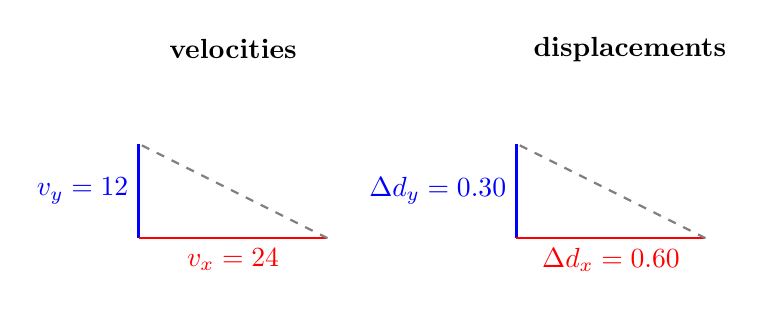
\begin{tikzpicture}[scale=1.2]
% velocity triangle
\draw[thick, blue] (0,0) -- (0,1) node[midway, left] {\(v_y = 12\)};
\draw[thick, red] (0,0) -- (2.0,0) node[midway, below] {\(v_x = 24\)};
\draw[thick, gray, dashed] (2.0,0) -- (0,1);
\node at (1.0,2.0) {\textbf{velocities}};
 
% displacement triangle
\begin{scope}[xshift=4cm]
\draw[thick, blue] (0,0) -- (0,1.0) node[midway, left] {\(\Delta d_y = 0.30\)};
\draw[thick, red] (0,0) -- (2.0,0) node[midway, below] {\(\Delta d_x = 0.60\)};
\draw[thick, gray, dashed] (2.0,0) -- (0,1.0);
\node at (1.2,2.0) {\textbf{displacements}};
\end{scope}
\end{tikzpicture}
\end{center}

\end{frame}

\begin{frame}{Example 2: Alternate Method — Using Similar Triangles}

\textbf{Since the directions are constant:}
\[
\frac{v_x}{v_y} = \frac{\Delta d_x}{\Delta d_y}
\]

\vspace{0.3cm}

\textbf{Substitute:}
\[
\frac{24}{12} = \frac{\Delta d_x}{0.30}
\Rightarrow \Delta d_x = 0.60 \text{ km [E]}
\]

\vspace{0.4cm}

\vspace{0.3cm}

\textbf{Conclusion:} the triangles are similar — so the ratio of sides gives the same result without using time!
\end{frame}

\begin{frame}{Example 2: Finding the Resultant Velocity}
\textbf{c) What velocity would you observe if you were standing at the school?}
 
\vspace{0.3cm}

\textbf{Given:}
\begin{itemize}
\item \(v_y = 12\) km/h [N]
\item \(v_x = 24\) km/h [E]
\end{itemize}
 

\textbf{Required:} \(v_T, \theta\)
 
\vspace{0.3cm}

\textbf{Analysis:} 
 
\[\vec{v_T} = \vec{v_y} + \vec{v_x}\]
 
\[v_T = \sqrt{v_y^2 + v_x^2}\]
 
\[\tan\theta = \frac{v_x}{v_y}\]
\end{frame}

\begin{frame}{Example 2: Finding the Resultant Velocity (continued)}
\textbf{Solution:}
 
\[v_T = \sqrt{(12)^2 + (24)^2} = 27 \text{ km/h}\]
 
\[\tan\theta = \frac{24}{12} = 2 \Rightarrow \theta = 63°\]
 
\begin{center}
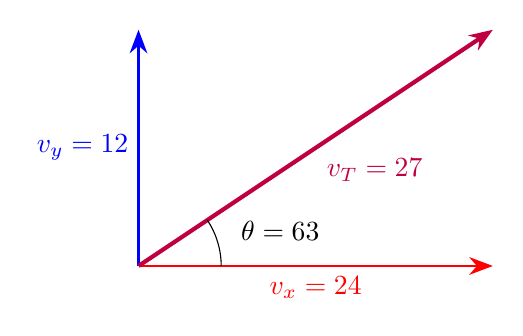
\begin{tikzpicture}[scale=1.5]
\draw[-{Stealth[length=3mm]}, thick, blue] (0,0) -- (0,2) node[midway, left] {\(v_y = 12\)};
 
\draw[-{Stealth[length=3mm]}, thick, red] (0,0) -- (3,0) node[midway, below] {\(v_x = 24\)};
 
\draw[-{Stealth[length=3mm]}, thick, purple, line width=1.5pt] (0,0) -- (3,2) node[midway, below right] {\(v_T = 27\)};
 
\draw (0.7,0) arc (0:33.7:0.7);
\node at (1.2,0.3) {\(\theta = 63°\)};
\end{tikzpicture}
\end{center}
\end{frame}

% --- SLIDE 1: why the boat can't make it directly across ---
\begin{frame}{Example 2: Finding the Angle}
\textbf{Concept:} The boat must aim upstream so its westward component cancels the eastward river current. Since the fixed "paddle rate" is $12 \text{km/h}$, this becomes our hypotenuse.

\begin{center}
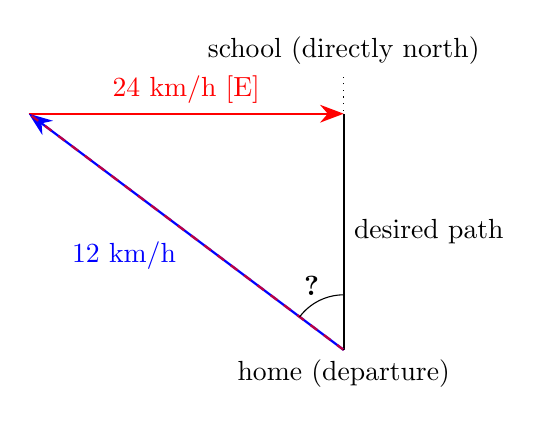
\begin{tikzpicture}[scale=1]
% coordinates
\coordinate (A) at (-2,2); % top-left
\coordinate (B) at ( 2,2); % top-right (top of vertical)
\coordinate (C) at ( 2,-1);% bottom-right (home / departure)

% top horizontal (24 km/h east)
\draw[-{Stealth[length=3mm]}, thick, red] (A) -- (B) node[midway, above] {\(24\ \text{km/h [E]}\)};

% vertical adjacent (straight up from departure)
\draw[thick] (C) -- (B) node[midway, right] {\(\text{desired path}\)};

% hypotenuse (boat heading = 12) drawn tip at A, tail at C
\draw[-{Stealth[length=3mm]}, thick, blue] (C) -- (A) node[midway, below left] {\(12\ \text{km/h}\)};

% resultant (dashed) from origin (C) to top-left (A) to emphasize tip-to-tail relation
\draw[dashed, thick, purple] (C) -- (A);

% angle marker with question mark
\draw pic["\textbf{?}", draw=black, angle eccentricity=1.3, angle radius=0.7cm]
  {angle=B--C--A};

% dotted line showing desired straight-across (north from departure)
\draw[dotted] (C) -- ++(0,3.5) node[above] {school (directly north)};

% labels for key points
\node[below] at (C) {home (departure)};

\end{tikzpicture}
\end{center}

\vspace{0.3cm}


\end{frame}

% --- SLIDE 2: visualizing why it’s impossible ---

\begin{frame}{Example 2: Finding the Angle (Impossible!)}

\textbf{Condition for a straight path:}
\[
\sin\theta = \frac{v_{\text{river}}}{v_{\text{boat}}}
\]

\vspace{0.3cm}
\textbf{Check:} 
\begin{center}\(\sin\theta = \dfrac{v_{\text{river}}}{v_{\text{boat}}} = \dfrac{24}{12} = 2\)
\end{center}

\vspace{0.3cm}
\textbf{Impossible!} Since \(\sin\theta\) cannot exceed 1, no such angle exists.

\vspace{0.3cm}
\textbf{Conclusion:} The river is flowing faster than the boat can paddle.  
The student \textit{must} drift downstream.

\end{frame}


% --- SLIDE 4: plane example intro ---
\begin{frame}{Example 3: Finding Angle (Possible this time!)}
\textbf{Scenario:} A pilot wants to fly due north, but there is a wind blowing 60 km/h from the west.  
The plane’s airspeed is 200 km/h.

\vspace{0.3cm}

\textbf{Question:} At what angle west of north must the plane head to actually travel due north?

\vspace{0.3cm}


\begin{center}
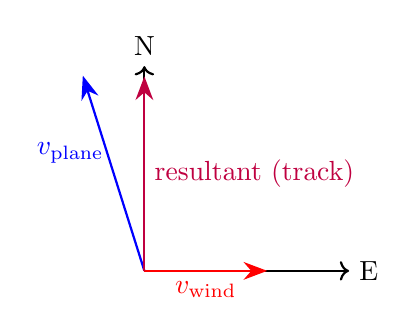
\begin{tikzpicture}[scale=1.3]
% axes
\draw[->, thick] (0,0) -- (0,2) node[above] {N};
\draw[->, thick] (0,0) -- (2,0) node[right] {E};
% plane velocity
\draw[-{Stealth[length=3mm]}, thick, blue, rotate=107.5] (0,0) -- (2,0) node[midway, above left] {\(v_{\text{plane}}\)};
% wind
\draw[-{Stealth[length=3mm]}, thick, red] (0,0) -- (1.2,0) node[midway, below] {\(v_{\text{wind}}\)};
% resultant (north)
\draw[-{Stealth[length=3mm]}, thick, purple] (0,0) -- (0,1.9) node[midway, right] {resultant (track)};
\end{tikzpicture}
\end{center}
\end{frame}


% --- SLIDE 5: plane solution + diagram ---
\begin{frame}{Example 3: Finding Angle (Possible this time!)}

\textbf{Given:}
\[
v_{\text{wind}} = 60 \text{ km/h [E]}, \quad v_{\text{plane}} = 200 \text{ km/h}
\]
\textbf{Required:} Heading angle \(\theta\)

\[
\sin\theta = \frac{v_{\text{wind}}}{v_{\text{plane}}}
= \frac{60}{200} = 0.30
\]
\[
\theta = \sin^{-1}(0.30) = 17.5^\circ
\]

\textbf{Therefore:} The pilot must head \(17.5^\circ\) west of north.

\vspace{0.4cm}

\end{frame}

\begin{frame}{What did we learn?}
\begin{itemize}
\item When given perpendicular vectors, the \textbf{Pythagorean theorem} and the \textbf{tangent function} can be used to find the resultant vector.  
\item River crossing problems are solved through \textbf{vector addition}, where the components represent independent motions in the x and y direction.  
\item The time it takes to complete each motion is the \textbf{same.}
\end{itemize}
\end{frame}

\begin{frame}{Practice Problems}
\textbf{Textbook Reference:} \\
Pages 66 – 74
 
\vspace{0.4cm}

\textbf{Practice Questions:}
\begin{itemize}
\item Pg 74 \#2
 
\item Pg 75 \#8 – 9
\end{itemize}
\end{frame}

\end{document}
